\documentclass[11pt,a4paper]{book}

\usepackage{Appunti}

\begin{document}
\title{Clean Code\\
\large{\textit{Robert C. Martin}}}
\author{Jacopo De Angelis}
\maketitle

\pagebreak
\tableofcontents
\pagebreak

\chapter{Clean code}
Il codice non finirà con l'era dell'autogenerazione da IA. Qualcuno dovrà creare le IA, qualcuno dovrà imparare come dare le specifiche. Il codice sarà sempre presente.

\section{Pessimo codice}
Una delle prime cause del pessimo codice è la fretta dettata dall'ansia. L'idea di dover far uscire il codice il prima possibile ci porta a commettere errori, commettere inesattezze. Quello è ciò che può portare a seri problemi successivamente, il rileggere il proprio codice scritto in maniere quantomeno esecrabili è una tortura. E ricordiamo che se si pensa "lo metto a posto dopo", dopo equivale a mai.

I rallentamenti derivanti da nuovo codice di bassa qualità sono esponenziali, lentamente la produttività crolla perchè operare sul codice precedente è sempre più complicato.
\begin{figure}[h!]
	\begin{center}
		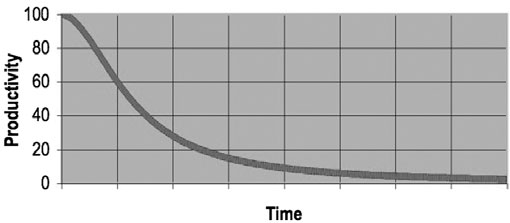
\includegraphics[scale=0.6]{img/001.png}
		\caption{Produttività vs tempo}
		\label{fig: 001}
	\end{center}
\end{figure}

Il che può portare ad un desiderio di ricreare da zero l'intera base del codice, cosa non solo dispendiosa ma che richiede anche molto tempo. I team si trovano a lavorare in parallelo, il nuovo team che ricrea tutto e integra il nuovo lavoro del vecchio team e, alla fine, ci si troverà nella stessa situazione.

\section{Scrivere buon codice}
Scrivere buon codice richiede disciplina nell'uso di molte piccole tecniche applicate in ogni singolo momento. Tutto questo richiede anche una parte di "senso estetico", un percepire il perchè un bel codice sia, appunto, bello.

Una regola che possiamo ereditare dai boy scout: lascia il campo più pulito di come l'hai trovato. Ad esempio: una variabile può avere un nome più autoesplicativo? Cambiala. Una funzione può essere spezzata in più funzioni elementari? Dividila.

\chapter{Nomi significativi}
\section{Usare nomi che rivelino l'intenzione}
Trovare nomi significativi non è semplice ma il tempo che prendono nel farlo è sicuramente meno di quello speso a decifrare nomi non chiari.

Ogni nome, che sia di variabile o di funzione, deve rispondere alle domande:
\begin{itemize}
	\item[] Cosa fa
	\item[] Perchè esiste
	\item[] Come viene utilizzata
\end{itemize}
Se un nome richiede un commento allora il nome è sbagliato.

Ad esempio
\lstinputlisting[language=java]{code/001}\label{code: 001}
d non dice molto come nome. Dovremmo scegliere un nome migliore, ad esempio
\lstinputlisting[language=java]{code/002}\label{code: 002}
Scegliere un nome che rivela un intento rende molto più semplice cambiare e comprendere un codice. Ad esempio cosa fa questo pezzo di codice?
\lstinputlisting[language=java]{code/003}\label{code: 003}
Il problema di questo codice non è la sua semplicità ma la sua capacità di avere un senso implicito. Ad esempio, le domande che ci possiamo porre sono:
\begin{itemize}
	\item[] Cos'è theList?
	\item[] Che significato ha l'elemento 0 di theList?
	\item[] Qual è il significato di 4?
	\item[] Come viene usata la lista ritornata?
\end{itemize}

Queste risposte dovrebbero essere nel codice. Immaginiamo ora di lavorare a campo minato. Rinominiamo la lista con gameBoard.

Ogni cella della board è rappresentata da un array, il valore alla posizione 0 è la posizione dello status della cella e se è 4 vuol dire "segnata". Già dando implicitamente queste notazioni possiamo migliorare il codice:
\lstinputlisting[language=java]{code/004}\label{code: 004}

Possiamo andare anche oltre e scrivere una semplice classe per le celle invece di avere degli int. Può includere una funzione con un nome che ne sveli l'intento per nascondere questo numero. Il risultato è:
\lstinputlisting[language=java]{code/005}\label{code: 005}

\section{Evitare la disinformazione}
Mai usare parole che non descrivono la realtà, ad esempio usare accountList solo se effettivamente ci troviamo davanti ad una List.

Non usare nomi che variano tra di loro per dei piccoli dettagli, ad esempio \emph{XYZControllerForEfficient\textbf{Handling}OfStrings} e \emph{XYZControllerForEfficient\textbf{Storage}OfStrings}

Avere una naming convention consistente è essenziale. Un pessimo esempio di uso è quello di o ed l minuscoli, pericolosamente simili a 0 e 1.

\section{Fare distinzioni significative}
Evitare nomi con degli errori di battitura intenzionali perchè si vogliono nominare due variabili allo stesso modo. Evitare anche nomi che non danno informazioni, ad esempio:
\lstinputlisting[language=java]{code/006}\label{code: 006}

Evitare nomi "che creano rumore", ad esempio ProductInfo e ProductData si differenziano per la seconda parola ma comunque non sappiamo cosa facciano.

Il tipo di entità non dovrebbe mai essere contenuto nel nome. NameString non ha senso, non ci chiederemmo mai se un semplice Name possa essere un float, questo perchè il nome stesso ci informa del suo contenuto.

Un esempio di confusione è:
\lstinputlisting[language=java]{code/007}\label{code: 007}
Come potremmo mai sapere quale funzione chiamare dal suo nome?

Distinguere sempre i nomi in modo da intuire immediatamente la loro funzione leggendoli.

\section{Usare nomi pronunciabili}
Devi poterlo pronunciare. Hai mai provato a discutere della funzione della classe Genymdhms (generation date, year, month, day, hour, minute, and second)? Spero di no.

Immaginiamo comparare questa classe
\lstinputlisting[language=java]{code/008}\label{code: 008}
con questa
\lstinputlisting[language=java]{code/009}\label{code: 009}

\section{Usare nomi ricercabili}
Le variabili con nome di una singola lettera vanno bene solo come variabili locali di un metodo, mai in altro modo, sarebbe impossibile cercarle altrimenti.

Compariamo
\lstinputlisting[language=java]{code/010}\label{code: 010}
con
\lstinputlisting[language=java]{code/011}\label{code: 011}

\section{Prefissi}
I prefissi erano utili anni fa, ormai sono abbastanza inutili.

\section{Interfacce e implementazione}
Ci sono due scuole di pensiero:
\begin{enumerate}
	\item Interfaccia che inizia con I, implementazione senza decorazioni (IClasse, Classe)
	\item Interfaccia senza decorazioni, implementazione con suffisso Imp (Classe, ClasseImp)
\end{enumerate}

É uguale.

\section{Evitare il mapping mentale}
Il significato dei nomi non deve essere chiaro solo a chi scrive ma anche a chi legge.

\section{Nomi delle classi}
Le classi dovrebbero essere nomi o frasi di sostantivi, evitare Manager, Processor, Data o Info. Una classe non dovrebbe essere un verbo

\section{Nomi dei metodi}
I nomi dovrebbero contenere un verbo che descrivere cosa fanno, ad esempio postPayment, deletePage o save.

Accessori, mutatori e predicati dovrebbero iniziare con get, set e is.

\section{Non usare nomignoli}
Non chiamare variabili, metodi e classi con nomi che utilizzano inside joke, riferimenti culturali o battute. Chiamare la funzione delete() holyHandGranade non è simpatico, è un inferno.

\section{Una parola per concetto}
Scegli una parola che esprima un concetto e mantienila. Ad esempio scegli tra fetch, retrieve e get e poi usa solo quella, non alternare tra le tre.

\section{Usare nomi del dominio della soluzione}
Meglio usare nomi che hanno un significato speciale nel caso sia quello il caso. Ad esempio, dire AccountVisitor vuol dire molto se si è a conoscenza del pattern visitor. I nomi che usano un lessico tecnico sono comodi.

\section{Usare nomi del dominio del problema}
Nel caso non ci siano nomi immediati da utilizzare facenti parte del dominio della soluzione, allora possiamo iniziare a guardare il dominio del problema.

\section{Aggiungere un contesto significativo}
Solitamente è meglio avere nomi che si spieghino da soli, in certi casi, però, ciò è difficile. Prendiamo ad esempio firstName, lastName, street, houseNumber, city, state e zipcode. Assieme sappiamo che sono un indirizzo ma presi singolarmente? Se vedessimo state usato da un'altra parte? In questo caso, allora, può essere accettabile usare, ad esempio addrFirstName, addrLastName, addrStreet, addrHouseNumber, addrCity, addrState e addrZipcode.

Non bisogna aggiungere del contesto a caso però, ad esempio dando a tutte le variabili un prefisso che descriva l'app.

\chapter{Funzioni}
La maggior parte delle regole di scrittura per le funzioni sono le stesse descritte dalle buone norme del \href{https://refactoring.guru/refactoring/techniques}{refactoring}.

\section{Corte}
Le funzioni dovrebbero essere lunghe massimo intorno alle 20 righe, nulla vieta di riuscire a ridurle ulteriormente però. Se è di più possiamo chiederci "è possibile estrarre una parte della funzione"?

Ad esempio la funzione
\lstinputlisting[language=java]{code/012}\label{code: 012}
è riscrivibile come
\lstinputlisting[language=java]{code/013}\label{code: 013}

\subsection{Blocchi e indentazione}
Se possibile sarebbe meglio ridurre i blocchi di indentazione a una sola linea, come abbiamo visto nel codice precedente, e possibilmente che chiami un'altra funzione per svolgere le sue funzioni.

Tutto ciò rende il codice snello e leggibile

\section{Fare una sola cosa}
Un metodo non deve fare tutto e male ma solo una cosa e farla bene. Un metodo che si occupa di una sequenza di passi avrà richiami a metodi che eseguono le subroutine ma non avrà altra logica al suo interno.

Se in una funzione vediamo più sezioni come dichiarazione, inizializzazione e scrematura come possiamo vedere qua
\lstinputlisting[language=java]{code/014}\label{code: 014}
vuol dire che probabilmente possiamo scomporla ulteriormente.

\section{Un livello di astrazione per funzione}
Ci si deve assicurare che una funzione sia ad un solo livello di astrazione. Non dovremmo mai avere funzioni ad alto livello di astrazione mischiate a codice a basso livello di astrazione, crea solo confusione e non rispetta il principio di responsabilità.

\subsection{Leggere il codice dall'alto verso il basso}
Primo avviso: questo si applica solo a linguaggi compilati e a linguaggi che si occupano dell'analisi di tutto il codice prima dell'esecuzione. In un linguaggio interpretato questa regola non si applica in quanto le funzioni devono essere descritte bottom-top.

Come regola di base dovremmo poter leggere il codice come una narrativa, dalla funzione principale a quelle ausiliarie, scendendo sempre più tra i vari livelli di astrazione.

\section{Controlli di flusso}
É difficile mantenere brevi gli switch e gli if/else. Possiamo però separare lo switch in una classe di basso livello e non vederlo mai ripetuto.

Consideriamo questo codice
\lstinputlisting[language=java]{code/015}\label{code: 015}
\begin{enumerate}
	\item è già grande e crescerà ancora di più all'aumentare delle tipologie di dipendenti
	\item fa più d una cosa
	\item viola il principio di singola responsabilità
	\item viola il principio open close\footnote{Le entità dovrebbero essere aperte per l'estensione, chiuse per le modifiche} perchè deve essere cambiata per ogni modifica nel dataset
\end{enumerate}

La soluzione a questo problema, ad esempio, è una \href{https://refactoring.guru/design-patterns/abstract-factory}{abstract factory}. La factory passerà l'istanza dei dipendenti e i vari metodi sono creati polimorficamente usando le interfacce.

Una regola possibile è che gli switch:
\begin{enumerate}
	\item devono compararire solo una volta
	\item devono sfruttare il polimorfismo
	\item devono essere nascosti tramite ereditarietà
\end{enumerate}
\lstinputlisting[language=java]{code/016}\label{code: 016}

\section{Usare nomi descrittivi}
Così come per le variabili, i nomi devono essere significativi. Meglio un nome lungo rispetto ad un nome che non spiega ciò che accade nel metodo.

Importante è avere una naming convention, anche non scritta, in modo che i nomi siano consistenti e che siano facilmente interpretabili.

\section{Argomenti delle funzioni}
Il numero ideale di argomenti per le funzioni è 0. Uno va bene, due accettabile, tre già è strano, quattro o più richiede una giustificazione seria.

\subsection{Forma comune per singolo argomento}
Ci sono due ragioni per passare un argomento:
\begin{itemize}
	\item stai ponendo delle domande su di esso
	\item stai operando su di esso
\end{itemize}

Un altra ragione è quella di generazione di un evento: il metodo ha in ingresso un argomento ma in uscita nessuno.

\subsection{Argomenti di guardia}
Sono brutti. Passare un boolean in una funzione come guardia per dire con che modalità eseguire la funzione è brutto a vedersi. Sarebbe meglio dividere la funzione in più metodi.

\subsection{Funzioni con due argomenti}
Una diade non per forza è negativa, ad esempio quando si crea un punto è necessario passare due variabili per gli assi x e y e ciò è giusto. Il problema è quando ci troviamo davanti ad altre forme come, ad esempio, \emph{assertEquals(expected, actual)}. Quale viene prima, quale dopo? Serve pratica perchè non c'è un ordine naturale.

Le soluzioni sono svariate, ad esempio estrarre un campo e renderlo appartenente alla classe.

\subsection{Oggetti come argomenti}
Spesso se vengono passati due o tre argomenti, questi saranno legati in qualche modo, probabilmente in un oggetto. In quel caso è meglio pensare di passare l'oggetto direttamente. Ad esempio qua è visibile la differenza di lettura dei due metodi.
\lstinputlisting[language=java]{code/017}\label{code: 017}

\subsection{Lista come argomento}
L'utilizzo delle liste opzionali di argomenti è molto comodo e in certi casi aiuta a tenere pulito il codice. Ad esempio
\lstinputlisting[language=java]{code/018}\label{code: 018}
A tutti gli effetti ha due argomenti ma a runtime può essere usato con infiniti argomenti.

\subsection{Verbi e parole chiave}
Usare una combinazione di verbi per le funzioni e sostantivi per gli argomenti può rendere le funzioni molto evocative. Ad esempio \emph{writeField(name)} subito fa capire che questo nome verrà scritto.

Codificare le variabili nel nome del metodo è anche un metodo interessante per renderla autodescrittiva. Tornando all'\emph{assertEquals(expected, actual)} di prima, quando sarebbe più immediato e meno confusa la sequenza se si chiamasse \emph{assertExpectedEqualsActual(expected, actual)}?

\section{Non devono avere effetti collaterali}
Gli effetti collaterali sono bugie. Una funzione dovrebbe fare una e una sola cosa, nascondere un effetto collaterale, ovvero l'agire su di una variabile esterna al suo scope, è un modo di farle fare più cose.

Ad esempio:
\lstinputlisting[language=java]{code/019}\label{code: 019}
Qua evidentemente inizializza la sessione quando la funzione dovrebbe solo validare l'utente. Questo va contro il principio di singola resposabilità

\section{Output}
Certi nomi possono confondere, portando a chiedersi se stiano parlando dell'input o dell'output. Ad esempio \emph{appendFooter(s)} attacca s ad un footer o attacca un qualche footer ad s? Solo guardando la firma del metodo si scopre che
\lstinputlisting[language=java]{code/020}\label{code: 020}
effettivamente attacca un footer al buffer passato.

Quello che abbiamo appena fatto è un controllo secondario, un qualcosa che può interrompere il flusso di programmazione.

In generale gli output dovrebbero essere evitati, se possibile è meglio far agire le funzioni sull'oggetto che le possiede.

\section{Separazione dei comandi}
Una funzione dovrebbe fare qualcosa o rispondere a qualcosa, non entrambe.

\section{Preferire le eccezioni al ritornare direttamente messaggi di errore}
Passare errori direttamente porta al doverli gestire subito, invece passare un'eccezione ha due benefici principali:
\begin{itemize}
	\item sono rapidi da usare e non si confonde ciò che può essere passato
	\item possono essere messi in calce al percorso di esecuzione
\end{itemize}

\subsection{Estrarre i blocchi try/catch}
Con ciò si vuole dire di non scrivere l'interno del blocco catch con tutti i suoi passaggi ma di portarlo fuori come metodo in modo da avere una struttura molto più compatta, leggibile e gestibile. Ricordiamo che le eccezioni vanno gestite il più vicino possibile alla fonte ma non per questo non possiamo mandarle alla funzione chiamante.
\lstinputlisting[language=java]{code/021}\label{code: 021}

\subsection{La gestione dell'errore è una sola cosa}
Le funzioni dovrebbero fare una sola cosa + la gestione dell'errore è una sola cosa = Una funzione che gestisce l'errore non dovrebbe fare altro. Ciò vuol dire che se in una funzione eiste la parola try dovrebbe essere la prima e niente dopo i blocchi catch e finally.

\subsection{Error.java e la dipendenza da esso}
Molti scrivono i messaggi di errore in una enumerazione da importare in ogni classe che la sfrutta. Risultato? Dipendenze ovunque ed essere costretti a modificare codice e ricompilare ogni volta.

Creare eccezioni figlie della classe Error invece rende il codice meno codipendente e più manutenibile.

\subsection{Non ripetersi}
Mai ripetere funzioni, piuttosto meglio importarle ma scrivere più volte lo stesso codice porta a dover debuggare più volte e c'è il rischio di riparare da una parte e non dalle altre.

\section{Programmazione strutturata}
Molti programmatori seguono il principio di Dijkstra: ogni funzione e ogni blocco deve avere una sola entrata e una sola uscita. Ciò vuol dire:
\begin{itemize}
	\item un solo return
	\item niente break o continue
	\item mai un goto
\end{itemize}

Questa regola perde di valore quando le funzioni sono molto brevi, questo perchè una sovraingegnerizzazione in un piccolo blocco di codice rischia di oscurare il vero significato dietro al metodo.

\section{Come si scrivono funzioni così?}
Ricorda: primo passaggio è la stesura, il successivo la pulizia. Va bene scrivere codice leggibile solo da te all'inizio, non devi lasciarlo così poi. Poco alla volta puoi pulirlo, renderlo perfetto.

\section{Esempio finale}
\lstinputlisting[language=java]{code/022}\label{code: 022}

\chapter{Commenti}
I commenti possono essere molto utili come anche superflui. Se imparassimo a scrivere codice comprensibile non ci servirebbe minimamente scrivere commenti. Spesso vengono inseriti per sopperire ad una mancanza del linguaggio.

Attenzione: commenti e documentazione non sono per niente la stessa cosa.

Tutto ciò vuol dire che nel momento nel quale si sente il bisogno di scrivere un commento bisogna chiedersi: posso scrivere il codice in modo che non serva?

Uno dei motivi principali di questa pratica è che il codice cambia, il commento spesso no.

I commenti non correggono del pessimo codice!

\section{Spiegati nel codice}
\lstinputlisting[language=java]{code/023}\label{code: 023}
Questo codice ha un commento perchè non è chiaro cosa faccia. É molto più semplice racchiudere la logica in un metodo a parte il cui nome spieghi cosa accade e poi usarlo, come ad esempio
\lstinputlisting[language=java]{code/024}\label{code: 024}
Ora è molto più chiaro e prende anche meno spazio

\section{Buoni commenti}
Alcuni commenti sono utili.

\subsection{Commenti legali}
Non è insolito che le aziende chiedano di inserire all'interno del codice un header con dei commenti riguardanti il copyright.

Questi commenti non dovrebbero essere contratti o lunghi quanto un libro di diritto. Dovrebbero rimandare alla licenza di riferimento, salvata da un'altra parte.

\subsection{Commenti informativi}
In certi casi è utile dare delle informazioni di base, per esempio la spiegazione di cosa ritorni un metodo
\lstinputlisting[language=java]{code/025}\label{code: 025}
Il problema è che certe informazioni andrebbero date, come sempre, tramite il nome della funzione. Ecco un caso leggermente migliore
\lstinputlisting[language=java]{code/026}\label{code: 026}
In questo caso il commento serve per dare la formattazione in maniera immediata

\subsection{Spiegazione d'intento}
In certi casi i commenti servono a spiegare quale fosse lo scopo di certe scelte di codice, ad esempio
\lstinputlisting[language=java]{code/027}\label{code: 027}
In questo modo lo sviluppatore rende nota la propria decisione e ciò che voleva raggiungere.

\subsection{Chiarimenti}
In certi casi è possibile scrivere commenti che spieghino al lettore una parte di codice 
\lstinputlisting[language=java]{code/028}\label{code: 028}
Chiaramente i commenti potrebbero essere sbagliati, per questo vanno presi con attenzione.

\subsection{Avvisare delle conseguenze}
In certi casi è meglio avvisare cosa accade usando certe feature, ad esempio
\lstinputlisting[language=java]{code/029}\label{code: 029}

\subsection{TODO}
\lstinputlisting[language=java]{code/030}\label{code: 030}
I todo sono comodi anche per capire perchè non bisogna fucilare il creatore di un metodo del genere. Sono un promemoria per noi e un avviso per gli altri.


\subsection{Aplificazione}
I commenti possono essere usati per esprimere l'importanza di parti non triviali o la cui importanza non è immediata.
\lstinputlisting[language=java]{code/031}\label{code: 031}

\subsection{Javadoc o simili}
Documentare in maniera corretta, utile e sufficiente tutto tramite le funzioni di documentazione è cosa buona e giusta. Ovviamente anche queste devono essere scritte bene ma possono contenere errori certe volte.

\section{Pessimi commenti}
\subsection{Ragionamenti generici}
\lstinputlisting[language=java]{code/032}\label{code: 032}
Ad esempio qua la fretta ha fatto sì che l'autore lasciasse un commento non chiaro. Chi è che carica i default? Quali sono i default? cc.

\subsection{Commenti ridondanti}
\lstinputlisting[language=java]{code/033}\label{code: 033}
Ad esempio qua il commento è già chiaro da ciò che c'è scritto nel metodo. Spesso un commento ridondante deriva dall'aver già scritto codice chiaro ma volerlo comunque commentare per paura.

\subsection{Commenti fuorvianti}
In certi casi, per puro errore umano, nonostante le buone intenzioni, si possono lasciare commenti fuorvianti. Anche un piccolo errore nella spiegazione del flusso dei dati può creare gravi problemi.

\subsection{Commenti obbligatori}
É ridicolo avere una regola che prescriva di scrivere per ogni funzione un javadoc o simili. 

\subsection{Commenti giornali}
In certi casi gli sviluppatori scrivono un giornale delle modifiche con data e cos'è stato fatto. É inutile, non aggiunge informazioni e diventa ancora più inutile coi sistemi di versionamento.

\subsection{Commenti di rumore}
Sono i commenti che non hanno nemmeno uno scopo, occupano spazio e basta.

\subsection{Rumore spaventoso}
C'è di peggio, ci sono i commenti che fanno ciò che devono ma che sono completamente inutili e poi ci sono quelli anche sbagliati.

\subsection{Indicatori per le parti}
Un commento tipo
\lstinputlisting[language=java]{code/034}\label{code: 034}
per indicare un blocco di codice è utile ad una prima vista ma in realtà se il codice è ben compartimentato non c'è da preoccuparsi per qualcosa del genere.

\subsection{Commenti per chiudere i blocchi}
\lstinputlisting[language=java]{code/035}\label{code: 035}
Questo modo di chiudere i blocchi per rendere più evidente a cosa si riferiscano è diventato completamente inutile grazie alle IDE. In più se un blocco è così vasto da non poterne riconoscere la fine, forse è meglio applicare un po' di refactoring.

\subsection{Attribuzione}
Scrivere in un commento l'autore di una parte di codice è inutile ed è reso semplice dal versionamento

\subsection{Codice rimosso tramite commento}
Eliminare del codice commentandolo, quindi in realtà lasciandolo in bella mostra, è rischioso, crea spreco di spazio e memoria e si accumula come pochi. Il versionamento aiuta a ricordare il codice cancellato, è inutile questa prassi.

\subsection{Commenti HTML}
\lstinputlisting[language=java]{code/036}\label{code: 036}
No.

\subsection{Informazione non locale}
Un commento è buono se si riferisce alla sua prossimità, fare riferimento a codice da altre parti è sbagliato.

\subsection{Troppe informazioni}
Non essere logorroico.

\subsection{Connessioni non ovvie}
\lstinputlisting[language=java]{code/037}\label{code: 037}
Ad esempio qua cos'è un byte filtro? Si collega al +1 o al *3?

Se un commento richiede una spiegazione allora è un pessimo commento

\subsection{Javadocs in codice non pubblico}
Se il codice deve essere acceduto dall'esterno allora va bene che sia commentato, altrimenti è superfluo.

\chapter{Formattazione}
\section{Formattazione verticale}
Il livello di dettaglio di una classe dovrebbe aumentare discendendo.
\begin{itemize}
	\item costanti
	\item variabili
	\item costruttori
	\item metodi pubblici
	\item metodi privati
	\item getter e setter
\end{itemize}

\subsection{Separazione delle parti}
Gli spazi tra i blocchi di codice sono utili per discriminare le parti del codice. L'apertura verticale separa i concetti.

\subsection{Associazione delle parti}
La densità verticale implica associazione, quindi le linee che verticalmente sono dense esprimono concetti legati

Se una parte ne chiama un'altra allora dovrebbero essere verticalmente vicine.

\section{Formattazione orizzontale}
Una volta il limite era 80 ma con gli schermi odierni il limite può essere alzato anche a 120. La regola da seguire, idealmente, è che a font standard non si debba mai scorrere a in orizzontale sullo schermo.

\subsection{Apertura orizzontale e densità}
Tra operatori e parti lo spazio serve, nella dichiarazione o nella chiamata di una funzione lo spazio tra nome della funzione e parentesi no, questo perchè sono strettamente legate.

\subsection{Allineamento orizzontale}
L'indentazione serve per rendere evidenti i blocchi di codice, aiutando così nella loro identificazione.

\section{Regole del gruppo}
Tutti abbiamo delle regole preferite ma se si lavora in gruppo allora si deve concordare su di uno stile unificato. Queste regole devono essere seguite e documentate.

\chapter{Oggetti e strutture dati}
\section{Astrazione}
Guardiamo i due listati seguenti. Entrambi rappresentano un punto del piano cartesiano, uno espone completamente la sua implementazione, l'altro lo nasconde.
\lstinputlisting[language=java]{code/038}\label{code: 038}
\lstinputlisting[language=java]{code/039}\label{code: 039}
La seconda classe nasconde come vengono salvate le sue variabili e, soprattutto, crea delle regole d'accesso ai dati. 

\section{Asimmetria dati/oggetti}
La differenza è:
\begin{itemize}
	\item gli oggetti nascondono i dati ed espone funzioni
	\item le strutture dati espongono i dati e non hanno funzioni significative
\end{itemize}

\section{Legge di Demetra}
\begin{itemize}
	\item ogni unità di programma dovrebbe conoscere solo poche altre unità di programma strettamente correlate
	\item ogni unità di programma dovrebbe interagire solo con le unità che conosce direttamente
\end{itemize}

Ovvero, data una classe C con un metodo f, questo metodo dovrebbe chiamare solo:
\begin{itemize}
	\item C
	\item Un oggetto creato da f
	\item Un oggetto passato come argomento ad f
	\item Un oggetto in un'istanza di C
\end{itemize}

\subsection{Incidenti ferroviari}
\lstinputlisting[language=java]{code/040}\label{code: 040}
Questo tipo di codice è chiamato incidente ferroviario perchè sembrano due treni che si sono scontrati e si sono accartocciati fino a diventare una cosa sola.

Questo stile di programmazione è da evitare, sarebbe meglio dividere le chiamate così
\lstinputlisting[language=java]{code/041}\label{code: 041}

Se questo insieme viola la legge di Demetra dipende se ctxt, Options e ScratchDir sono oggetti o strutture dati. Se sono oggetti, le loro strutture interne dovrebbero essere nascoste e quindi la conoscenza dell'interno è chiaramente una violazione della legge. Se sono strutture dati senza comportamenti, allora esporranno naturalmente le loro strutture interne, e quindi la legge non si applica.

\subsection{Ibridi}
Certe volte vengono create classi che sono anche strutture dati, presentano varaibili pubbliche e private, accessori di ogni tipo e funzioni significative. Sono da evitare, è un caso di \href{https://refactoring.guru/smells/feature-envy}{"feature envy"}, ovvero metodi che chiamano funzioni o attributi di altre classi più della propria.

\subsection{Nascondere le strutture}
Se comunichiamo con un oggetto dovremmo dirgli di fare qualcosa, non dovremmo chiedere i suoi dettagli interni.

Ad esempio, nel caso delle chiamate di prima, ottenevamo il percorso assoluto di un file, un errore gigantesco. In più cosa dobbiamo farci? Se volessimo creare un nuovo file non sarebbe meglio fare così?
\lstinputlisting[language=java]{code/042}\label{code: 042}
In questo modo i dettagli sull'implementazione sarebbero nascosti.

\section{Data Transfer Object (DTO)}
un DTO è una struttura dati molto utile, specialmente quando si comunica col database o si devono elaborare dei dati prima di presentarli. I loro campi sono pubblici e utilizzabili.

Sono comuni anche i "bean", oggetti con variabili private ma con getter e setter.
\lstinputlisting[language=java]{code/043}\label{code: 043}

\subsection{Active records}
Sono tipi speciali di DTO. Hanno strutture dati con variabili pubbliche o accessibili ma solitamente hanno metodi come salva e trova. Spesso sono traduzioni dirette del database.

\chapter{Gestione errori}
La gestione errori è importante ma se offusca la logica allora c'è un problema.

\section{Usare le eccezioni invece del return}
Una volta, quando non c'era una gestione delle eccezioni come ora, si usavano dei flag per segnalare gli errori. Al giorno d'oggi possono essere sollevate eccezioni che rendono la vita molto più semplice e, soprattutto, possono rendere il codice più comprensibile.

\section{Scrivere il blocco Try-Catch-Finally prima di tutto}
Il blocco catch deve permettere l'uscita dal metodo in uno stato consistente, indipendentemente da cosa sia successo nel try.

\section{Usare eccezioni non controllate}
Le eccezioni controllate violano il principio Open/closed perchè creano più uscite. Se si solleva un'eccezione e viene mandata tre livelli sopra allora si dovrà inserire nell'intestazione di tutti i metodi della catena.

\section{Offrire un contesto con le eccezioni}
Le eccezioni dovrebbero offrire abbastanza informazioni da consentire di comprendere cosa le abbia scatenate. Lo stacktrace è utile ma non è l'unica fonte, anche un messaggio significativo è ottimo.

\section{Definire le classi di eccezioni in termini dei bisogni del chiamante}
Ci sono molti modi per classificare gli errori. Possiamo classificarli dalla loro fonte o per il loro tipo. La cosa, però, realmente più importante in questo contesto è "come sono catturati"?

Ora vediamo un esempio di pessima classificazione in una libreria:
\lstinputlisting[language=java]{code/044}\label{code: 044}

Questo blocco di codice contiene molte ripetizioni. In questo caso possiamo racchiudere le eccezioni in un tipo generico che però contenga una descrizione dell'errore. 

\lstinputlisting[language=java]{code/045}\label{code: 045}
Rinchiudere in un wrapper le eccezioni derivanti da una libreria di terze parti può essere molto comodo. In più permette di non dover dipendere dalle scelte di design di qualcun altro.

\section{Non ritornare null}
Mai e poi mai ritornare null. Rendere un programma null safe è essenziale per evitare la maggior parte degli errori.

Usare un optional o, ad esempio, una emptyList, sono metodi per poter permettere al flow del programma di non incontrare una NullPointerException.

\chapter{Limiti}
\section{Usare codice di terze parti}
Speso nella scrittura del codice da poter implementare da terze parti si pensa all'uso più generico possibile che può essere fatto mentre l'utente ha bisogno di un uso specifico. In cosa si traduce questo? Nel dover pensare a come rendere specifico questo codice per evitare problemi. Ad esempio
\lstinputlisting[language=java]{code/046}\label{code: 046}
Il codice non è perfettamente leggibile, il typecast è una pezza messa alla generalità della mappa. Potrebbe essere risolto rendendo specifica la mappa
\lstinputlisting[language=java]{code/047}\label{code: 047}
Ma in questo caso non verrebbe risolto un problema essenziale: Map fornisce più funzioni di quelle che vogliamo, tra cui clear, attivabile da chiunque. Come possiamo allora nascondere questo problema implementativo? Semplice, mascherandolo in una classe apposita che si occupi di typecast, gestione degli accessi ecc.
\lstinputlisting[language=java]{code/048}\label{code: 048}
In questo modo l'utente non deve preoccuparsi di certi dettagli implementativi, di dover stare attento a cosa venga ritornato ecc. ma invece può usare in maniera naturale la classe Sensor.

\section{Esplorare e comprendere i confini}
Quando ci si trova a implementare una libreria di terze parti si possono passare giorni a leggerne la documentazione ma non è detto che ciò che si pensa faccia la libreria e ciò che fa veramente siano la stessa cosa. Per questo motivo, prima di generare bug complicati, sarebbe meglio creare delle suite di test per testare le funzioni richieste alla libreria e vedere se il comportamento atteso è quello effettivo o no. Questo metodo, per quanto tedioso, può risparmiare molto tempo più avanti.

\subsection{Conoscere log4j e slf4j}
Per fare un esempio, uno potrebbe pensare "beh, se inizializzo il logger e dico di loggare sono a posto" e invece no
\lstinputlisting[language=java]{code/049}\label{code: 049}
Questo codice restituisce un errore in quanto il Logger ha bisogno di un appender. Allora viene aggiunto ciò
\lstinputlisting[language=java]{code/050}\label{code: 050}

Ma a quanto pare ha bisogno di un output stream, allora aggiungiamo
\lstinputlisting[language=java]{code/051}\label{code: 051}
E ora funziona! Ora però rimuovendo l'output stream continua a funzionare ma non rimuovendo il pattern, strano. Studiando ancora la configurazione scopriamo che semplicemente il Logger non era configurato, cosa che non è altamente intuitiva. Ancora un po' di ricerca e raggiungiamo questa classe di test che rappresenta la conoscenza acquisita
\lstinputlisting[language=java]{code/052}\label{code: 052}

\section{I test di apprendimento sono ottimi}
Questi test, oltre a darci un'ottima conoscenza la prima volta, ci permettono di tenere sotto controllo anche eventuali aggiornamenti. Infatti ad ogni nuova release ci basta far partire nuovamente i test per controllare che tutto sia come prima. In questo modo abbiamo anche un ottimo rientro sull'investimento.

\chapter{Unit test}
\section{Le tre leggi del test driven development}
\begin{enumerate}
	\item Non scriverai codice in produzione fino a quando non avrai scritto il codice per testarlo
	\item Non scriverai più di un test che debba fallire e la non compilazione è un fallimento
	\item Non scriverai più codice di quanto non sia strettamente necessario per passare il test
\end{enumerate}

\section{Mantenere i test puliti}
Non bisogna minimamente pensare che i test non debbano essere scritti con meno cura rispetto al codice originale


\end{document}